%
% krbeispiele.tex
%
% (c) 2021 Prof Dr Andreas Müller, OST Ostschweizer Fachhochschule
%
\begin{frame}[t]
\frametitle{Konvergenzradius --- Beispiele}
\vspace{-20pt}
\begin{columns}[t,onlytextwidth]
\begin{column}{0.48\textwidth}
\begin{block}{Exponentialreihe}
\vspace{-20pt}
\begin{align*}
e^z &= \sum_{k=0}^\infty \frac{z^k}{k!}
\\
\uncover<2->{
\frac1k\log k!
}
&\uncover<3->{=\frac1k\sum_{x=1}^k {\color{blue}\log x}}
\uncover<6->{>\frac1k\int_1^k{\color{red}\log x}\,dx}
\\
&
\ifthenelse{\boolean{presentation}}{
\only<7>{=\frac1k[x\log x -x]_1^k}
}{}
\only<8->{=
\log k -1 +\frac1k}
\uncover<9->{\to \infty\phantom{\frac1k}}
\\
\uncover<10->{(k!)^{\frac1k}
&\to\infty}\uncover<11->{ \quad\Rightarrow\quad R = \infty}
\end{align*}
\vspace{-40pt}
\begin{center}
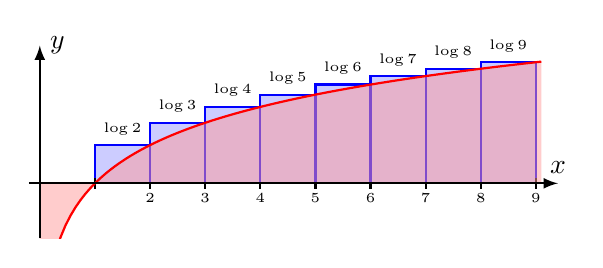
\begin{tikzpicture}[>=latex,thick,scale=0.7]
\uncover<4->{
\foreach \x in {2,...,9}{
	\fill[color=blue!20] ({\x-1},0) rectangle ({\x},{ln(\x)});
	\draw[color=blue] ({\x-1},0) rectangle ({\x},{ln(\x)});
	\node at ({\x-0.5},{ln(\x)}) [above] {\tiny $\log\x$};
	\draw (\x,-0.1) -- (\x,0.1);
	\node at (\x,0) [below] {\tiny$\x$};
}
\draw (1,-0.1) -- (1,0.1);
\uncover<5->{
\begin{scope}
	\clip (0,-1) rectangle (9.5,2.5);
	\fill[color=red!40,opacity=0.5] (0,0) -- (0,-1)
		-- plot[domain=0.1:9.1,samples=100] ({\x},{ln(\x)})
		-- (9.1,0) -- cycle;
	\draw[color=red] plot[domain=0.1:9.1,samples=100] ({\x},{ln(\x)});
\end{scope}
}
\draw[->] (-0.2,0) -- (9.4,0) coordinate[label={$x$}];
\draw[->] (0,-1) -- (0,2.5) coordinate[label={right:$y$}];
}
\end{tikzpicture}
\end{center}
\end{block}
\end{column}
\begin{column}{0.48\textwidth}
\uncover<12->{%
\begin{block}{Geometrische Reihe}
\vspace{-15pt}
\begin{align*}
\uncover<13->{
\frac{1}{{\color{blue}1}-z}
&=
\sum_{k=0}^\infty
z^k}
\\
\uncover<14->{
a_k&=1}
\uncover<15->{\quad\Rightarrow\quad
|a_k|^{\frac1k}=1}
\\
\uncover<16->{
\limsup_{k\to\infty} &= |a_k|^{\frac1k}=1}\uncover<17->{ = \frac1R}
\uncover<18->{\quad\Rightarrow\quad R=1}
\end{align*}
%\uncover<19->{Polstelle bei $z=1$ limitiert Konvergenzradius}
\vspace{-20pt}
\begin{center}
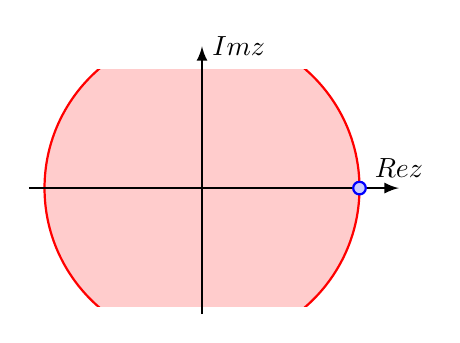
\begin{tikzpicture}[>=latex,thick]
\begin{scope}
\clip (-2.2,-1.5) rectangle (2.2,1.5);
\fill[color=red!20] (0,0) circle[radius=2];
\draw[color=red] (0,0) circle[radius=2];
\end{scope}
\draw[->] (-2.2,0) -- (2.5,0) coordinate[label={$\operatorname{Re}z$}];
\draw[->] (0,-1.6) -- (0,1.8) coordinate[label={right:$\operatorname{Im}z$}];
\fill[color=blue!20] (2,0) circle[radius=0.08];
\draw[color=blue] (2,0) circle[radius=0.08];
\end{tikzpicture}
\end{center}
\end{block}}
\end{column}
\end{columns}
\end{frame}
